%%%%%%%%%%%%%%%%%%%%%%%%%%%%%%%%%%%%%%%%%
% FRI Data Science_report LaTeX Template
% Version 1.0 (28/1/2020)
% 
% Jure Demšar (jure.demsar@fri.uni-lj.si)
%
% Based on MicromouseSymp article template by:
% Mathias Legrand (legrand.mathias@gmail.com) 
% With extensive modifications by:
% Antonio Valente (antonio.luis.valente@gmail.com)
%
% License:
% CC BY-NC-SA 3.0 (http://creativecommons.org/licenses/by-nc-sa/3.0/)
%
%%%%%%%%%%%%%%%%%%%%%%%%%%%%%%%%%%%%%%%%%


%----------------------------------------------------------------------------------------
%	PACKAGES AND OTHER DOCUMENT CONFIGURATIONS
%----------------------------------------------------------------------------------------
\documentclass[fleqn,moreauthors,10pt]{ds_report}

\usepackage[english]{babel}
\usepackage{svg}
\graphicspath{{fig/}}
\usepackage{xcolor}




%----------------------------------------------------------------------------------------
%	ARTICLE INFORMATION
%----------------------------------------------------------------------------------------

% Header
\JournalInfo{FRI Data Science Project Competition 2025}

% Interim or final report
\Archive{Final report} 

% Article title
\PaperTitle{From Cell Towers to Traffic: Harnessing Cellular Network Data for Transport Modeling in Slovenia} 

% Authors (student competitors) and their info
\Authors{Muhammad Ali, Juan Osorio, Kristjan Sever}

% Advisors
\affiliation{\textit{Advisors: prof. dr. Tomaž Curk, Leon Hvastja}}

% Keywords
\Keywords{Cellular Mobility Data, Trajectory Denoising, Transport Mode Inference}
\newcommand{\keywordname}{Keywords}

%----------------------------------------------------------------------------------------
%	ABSTRACT
%----------------------------------------------------------------------------------------

\Abstract{
This project analyzes anonymized cellular mobility traces derived from cellular networks to uncover transportation patterns across Slovenia. Given the high spatial and temporal noise typical of such datasets, we developed a multi-stage denoising pipeline combining tower proximity filtering, heuristics-based smoothing (Zheng’s algorithm), and a rolling median speed filter. After cleaning, trajectories were aggregated spatially and temporally using a zone-based binning system to construct hourly transition matrices. 
Building on these transition matrices, we applied spectral clustering to uncover latent regional communities and simultaneously derived per‐zone×hour features for unsupervised mode inference. Using clustering on log‐transformed features—refined by smoothing—we recovered walking, cycling, driving, and other shares that broadly mirror existing survey‐based patterns. Our work demonstrates the feasibility of extracting high-resolution mobility signals from raw mobile network data using scalable preprocessing, while also exposing current limitations in sampling rate, mode discrimination, and reliance on heuristic thresholds.
}

%----------------------------------------------------------------------------------------

\begin{document}

% Makes all text pages the same height
\flushbottom 

% Print the title and abstract box
\maketitle 

% Removes page numbering from the first page
\thispagestyle{empty} 

%----------------------------------------------------------------------------------------
%	ARTICLE CONTENTS
%----------------------------------------------------------------------------------------

\section*{Introduction}
Urban mobility underpins economic vitality, environmental sustainability, and quality of life in modern urban centers. Yet, traditional tools for measuring travel behavior—household surveys, manual counts, and fixed sensors—are costly, infrequent, and spatially or temporally limited. As a result, planners often lack the real-time, high-resolution data needed to adapt infrastructure and policy to evolving demand.

Mobile-network traces (cellular “pings”) could potentially fill this gap: they record location updates continuously across all mobile devices, offering unprecedented coverage. However, these data comes with three major challenges:

\begin{itemize}[nosep]
  \item \textbf{Spatial uncertainty.}  Tower‐based positioning introduces jitter and fallback clusters at mast sites, destroying true movement paths.  
  \item \textbf{Temporal artifacts.}  Irregular sampling intervals obscure trip boundaries.  
  \item \textbf{Scale.}  Hundreds of millions of pings per day nationwide.  
\end{itemize}

Although cellular data presents significant noise challenges, as others have already demonstrated, \cite{urbansensing}  substantial mobility insights can still be extracted through appropriate processing techniques~\cite{wang2010transport,asgari2016ctmapper}.

In this work, we address two core problems:
\begin{enumerate}[nosep]
  \item \emph{Data hygiene and structuring:} How can we turn noisy, large‐scale cellular pings into interpretable summaries of movement?  
  \item \emph{Mode and flow inference:} Without ground-truth labels, how can we infer travel modes (walk, bike, car, others) and estimate flows?
\end{enumerate}

To solve these challenges, we devise a unified pipeline that cleans and structures raw pings, infers travel modes, and extracts hourly Origin-Destination (OD) flows.

%------------------------------------------------

\section*{Methods}

\subsection*{Denoising}
As illustrated in Figure~\ref{fig:trace}, the raw location data exhibits substantial noise, manifesting itself as sudden jumps, erratic oscillations, and dense clusters of redundant pings. To ensure the spatial-temporal validity of the data and to enable reliable mobility analysis, a multi-stage denoising pipeline was developed. Each stage targets a specific type of artifact, and their combination progressively transforms noisy mobile devices trajectories into cleaner and interpretable data.

\begin{figure}[hbt]\centering
	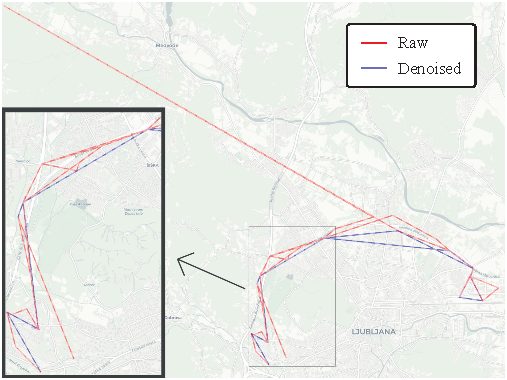
\includegraphics[width=\linewidth]{fig/traces_final.pdf}
	\caption{Map depicting raw (red) and denoised (blue) trajectories from the same device. Though containing fewer positions, denoised captures the true trajectory.}
	\label{fig:trace}
\end{figure}

\subsubsection*{Tower Proximity}
To remove “fallback” pings at mast locations, we used data from Slovenian tower registry. We build a \texttt{cKDTree} of tower coordinates, query each ping’s nearest‐tower angular distance, and flag pings within 3m. This threshold captures typical mast‐fallback jitter while preserving genuine movement and preventing false “stops.”


\subsubsection*{Repeated Coordinates}
Devices occasionally emit duplicate pings from the exact same location, typically during long periods of physical inactivity or when cell towers fail at locating the device. To address this, all coordinate pairs (\texttt{lat}, \texttt{lon}) that appear more than a fixed threshold are considered invalid and are dropped. This heuristic targets infrastructural or environmental signal anomalies (e.g., default fallback locations such as the cell-towers position or parking lots).

\subsubsection*{Yu Zheng's Algorithm}
The core of our denoising logic builds upon the trajectory-smoothing heuristics proposed by Yu Zheng~\cite{yuzheng}. This method evaluates the geometric plausibility of each geographic point within its temporal and spatial context for each device, using three key thresholds: speed, angular deviation, and time. \\

\noindent\textbf{Speed Constraint.} \\
For every point \( p_t \), we compute its instantaneous speed relative to its predecessor using the haversine formula. This distance is divided by the time elapsed between pings to yield speed. If the result exceeds a certain threshold, the point is flagged as implausible and removed. This method deals with high-speed displacements characteristic of position jitter. \\

\noindent\textbf{Angular Constraint.} \\
Points forming abrupt, implausible turns are identified using a three-point angle test. For every triplet \((p_{t-1}, p_t, p_{t+1})\), we compute the angular deviation between the incoming and outgoing bearings. If the angle computed exceeds a predefined threshold, the middle point \(p_t\) is discarded, since such abrupt turns are unlikely in real trajectories.\\

\noindent\textbf{Time Constraint.} \\
To enforce a minimum sampling interval and reduce clustering, pings spaced by less than 10 seconds are evaluated as potential duplicates. When these points do not contribute new directional or positional information, they are removed. This rule helps suppress dense bursts of low-information records, reducing over-representation of stationary or slowly moving devices.

\subsubsection*{Sliding Window Median Filter}
The sliding window median filter is a technique that smooths short-term spikes in the speed profile of each device. It operates on a per-device basis using a centered rolling median of the instantaneous speed values over a configurable window size. Any point whose speed exceeds a pre-defined threshold compared to the local median is discarded. 

This method helps to mitigate isolated noise bursts that may pass the previous Zheng-based denoising. In practice, it is especially effective in removing erratic high-speed anomalies or position glitches that appear intermittently across a trajectory.

\subsubsection*{Minimal Viable Points per Device}

Finally, any device contributing fewer than 3 valid pings after denoising is dropped entirely. Such trajectories lack sufficient information for any meaningful analysis, and retaining them would only introduce noise in aggregate statistics.

The average outcome of the denoising pipeline can be found on Table \ref{tab:data_reduction}, meanwhile, the used parameters in each step can be consulted on Table \ref{tab:denoise_params}. 


\begin{table}[hbt]
    \caption{Average data reduction through denoising pipeline.}
    \centering
    \begin{tabular}{l | r r}
        \toprule
        Processing Step & Data Points & Unique Devices \\
        \midrule
        Raw data & 128 M & 753 K \\
        Tower proximity & 125 M & 749 K \\
        Repeated coords & 114 M & 737 K \\
        Zheng denoise & 91 M & 626 K \\
        Sliding window & 85 M & 621 K \\
        Device removal & 84 M & 501 K \\
        \bottomrule
    \end{tabular}
    \label{tab:data_reduction}
\end{table}

\begin{table}[hbt]
    \caption{Parameters used in each denoising step.}
    \centering
    \renewcommand{\arraystretch}{1.2} % adds vertical spacing
    \begin{tabular}{lll}
        \hline
        \textbf{Step} & \textbf{Parameter} & \textbf{Value} \\
        \hline
        Tower proximity  & Tower radius       & 3.0 m \\
        Repeated coords  & Count threshold    & 150000 \\
        Zheng denoise    & Speed threshold    & 30.0 m/s \\
                         & Angle threshold    & 30.0° \\
                         & Time threshold     & 10 s \\
        Sliding window   & Window size        & 5 \\
                         & Speed threshold    & 40.0 m/s \\
        Device filtering & Minimum points     & 3 \\
        \hline
    \end{tabular}
    \label{tab:denoise_params}
\end{table}



\subsection*{Spatial Zoning and Temporal Binning}

Each mobile data ping is assigned to a predefined spatial zone using a spatial join against a polygonal grid covering Slovenia. The Figure \ref{fig:bins} shows that data encompasses 950 out of 2680 zones.

\begin{figure}[hbt]\centering
	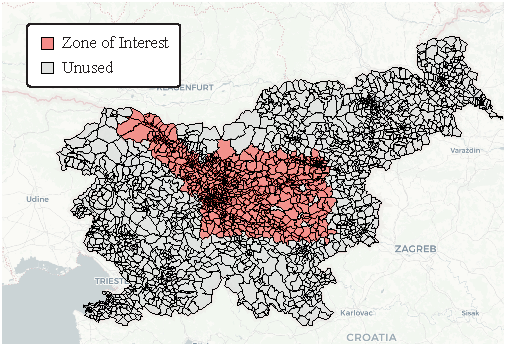
\includegraphics[width=\linewidth]{fig/binned.pdf}
	\caption{Zones of interest highlighted}
	\label{fig:bins}
\end{figure}

Additionally, every point is assigned to a fixed-size time bin, allowing for aggregated temporal analyses. For this project, 60-minute intervals were used as the granularity. This allows for efficient construction of OD matrices.

\subsection*{Transition Matrices}
We created transition matrices to capture user movement between zones, where each element in the matrix represents transitions from zone-to-zone during each hour on a day.

Initially, we counted all transitions within each hour, but stationary users dominated the data. We experimented with several alternative counting rules and filtering methods before refining our approach to register users based on their predominant zone in each time bin, counting only transitions between consecutive time bins.

This time-binned approach filtered problematic data with large temporal gaps, improving reliability by eliminating speculative transitions.

\subsection*{Bin‐Level Feature Extraction}
\label{sec:binning_insights}

After assigning every ping to a spatial zone and an hourly time‐bin, we assemble a feature table summarizing local movement patterns.  First, we compute per‐ping speeds, by calculating the distance using haversine formula, over consecutive timestamps (with device‐change resets to avoid cross‐device leakage).  Next, for each \((\mathrm{zone\_id},\mathrm{time\_bin})\) cell we aggregate:

\begin{itemize}[nosep]
  \item \textbf{Speed Metrics:} Mean, median, min, max, variance and interquartile range of instantaneous speeds.
  \item \textbf{Density \& Entropy:} Total pings, unique devices, pings per device, and Shannon entropy of device counts to distinguish crowded hubs from infrequent visitors.
  \item \textbf{Dwell Time:} Per‐device stop durations (max–min timestamp) summarized by mean, median, min and max.
  \item \textbf{Transition Profiles:} Counts and mean speeds of entries/exits per zone, plus entropy over next‐zone destinations.
  \item \textbf{Temporal Flags \& Priors:} Binary indicators for morning/evening commute and late‐night bins.
\end{itemize}

This produces matrices of roughly 22K Zones$\times$Time rows with 27 features each, serving as the input for our cluster-based classification and Hidden Markov Model. By compressing millions of raw pings into summarized statistics, this step bridges low‐level trajectory denoising and high‐level mode‐inference.

%------------------------------------------------
\section*{Results}

\subsection*{Zone‐to‐Zone Flows}
We constructed daily OD matrices that aggregate zone-to-zone transitions. Each OD matrix counts the number of users transitioning from zone $i$ to zone $j$ between two consecutive time bins.

To uncover latent spatial structure, we applied spectral clustering to a symmetrized version of the log-transformed OD matrix~\cite{louail2015spatial}. This revealed approximately 5–6 coherent zone clusters, as shown in Figure~\ref{fig:cluster_map}.


When plotted spatially, the clusters revealed regional commuting basins. For instance, Ljubljana and its immediate surroundings formed a highly connected cluster. These findings suggest that clustering over the OD patterns can reveal latent urban structure, even without explicit land-use data.

\begin{figure}[ht]
  \centering
  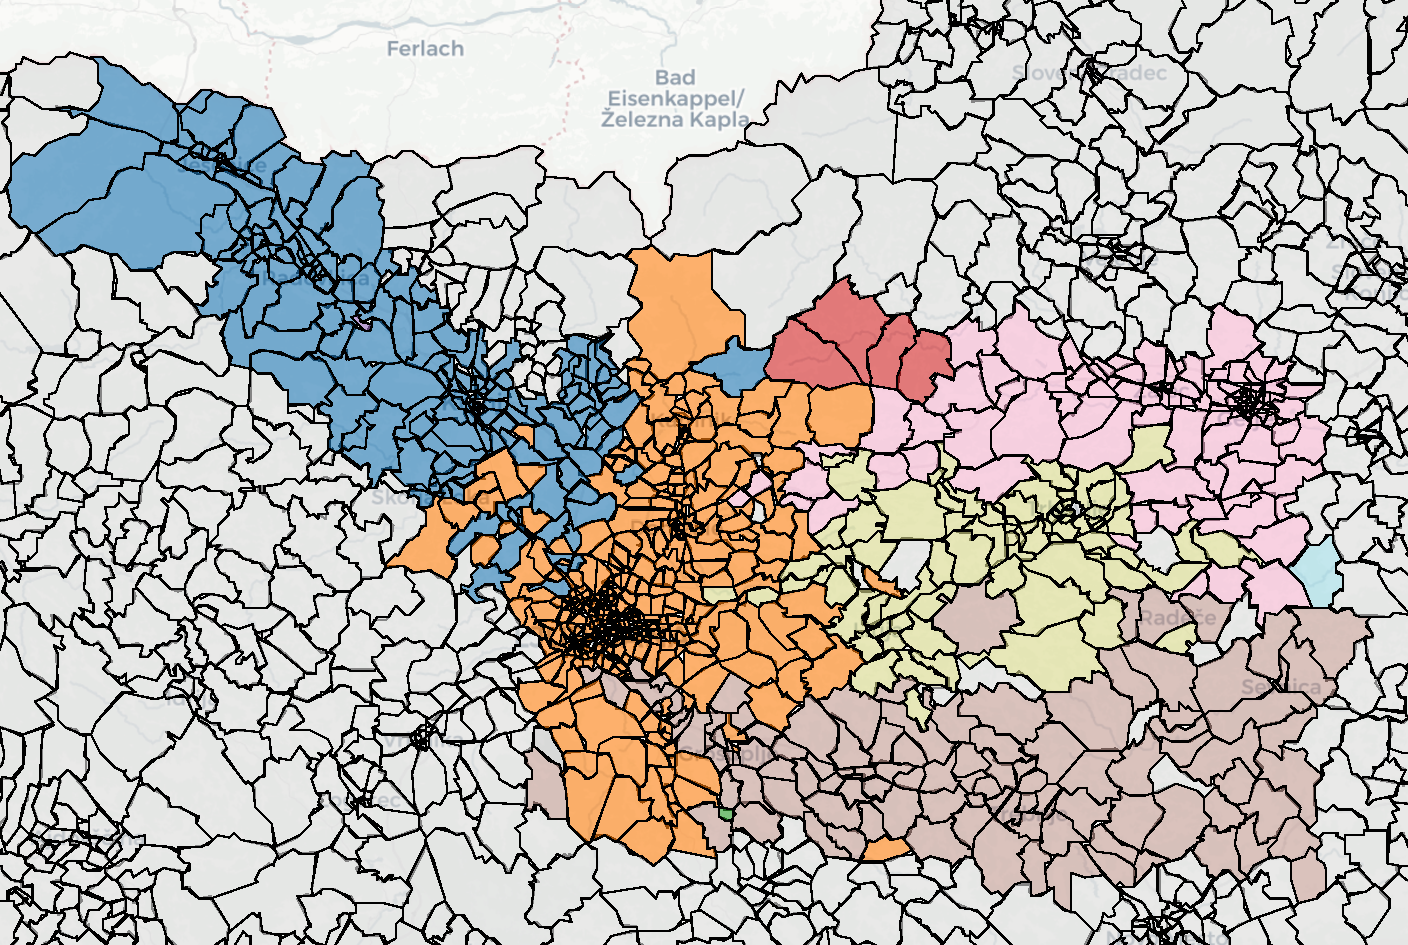
\includegraphics[width=0.85\linewidth]{fig/cluster_map.pdf}
  \caption{Map of clustered zones derived from OD spectral clustering where community-like internal flow occurs.}
  \label{fig:cluster_map}
\end{figure}

\subsection*{Mode Inference}

Our raw data contains no ground-truth labels, so after clustering, we need a principled way to assign each cluster to a transport mode~\cite{dutta2023transport}.
  We do this by ordering the four K‐Means centroids by their mean log‐speed (with dwell time as a secondary cue) and mapping:
\[
\begin{aligned}
  \text{Cluster 1: } &\underbrace{\text{slowest centroid}}_{\text{lowest speed}}
    \quad\longrightarrow\quad \text{Walk},\\
  \text{Cluster 2: } &\text{next slowest centroid}
    \quad\longrightarrow\quad \text{Bike},\\
  \text{Cluster 3: } &\text{next fastest centroid}
    \quad\longrightarrow\quad \text{Car},\\
  \text{Cluster 4: } &\underbrace{\text{Others centroid}}_{\text{mixed speed}}
    \quad\longrightarrow\quad \text{Others}.
\end{aligned}
\]

This simple heuristic leverages the fact that typical walking speeds (~1–2 m/s), cycling (~3–5 m/s), driving ($>10$m/s), and others (mixed speeds) separate out in the log-speed domain. Figure~\ref{fig:global_kmeans} shows the percent share of all Zone$\times$Hour bins assigned by raw K-Means plus this centroid‐based labeling.

\begin{figure}[ht]
  \centering
  \includesvg[width=1.0\linewidth]{fig/global_kmeans.svg}
  \caption{Global mode distribution after K-Means clustering and mapping clusters→modes by ascending centroid speed.}
  \label{fig:global_kmeans}
\end{figure}

\vspace{1ex}
\noindent\textbf{Key findings:}
\begin{itemize}[nosep]
  \item \textbf{Mode composition.}  Walk (43.6\%), Bike (3.1\%), Car (42.9\%), Others (10.4\%).
  \item \textbf{Smoothing consistency.}  Enforcing temporal coherence via HMM smoothing (self‐transition ≈0.9) changes these shares by $<$0.5\% increase, showing the unlabeled clustering is already capturing the bulk of mode separation.  
  \item \textbf{Reduced noise.}  Although aggregate shares stay similar, HMM smoothing removes isolated one‐hour changes of mode, creating more realistic contiguous mode segments.
\end{itemize}

Overall, our centroid‐based mapping of unlabeled clusters plus HMM smoothing provides a lightweight yet effective way to recover plausible travel modes from discretized cellular data.


\section*{Discussion}

Although they compose a rational step forward for modeling, both the denoising and binning are computationally tasking and optimizations/shortcuts had to be implemented which may introduce artifacts in both cases (e.g., Not removing subsequent noisy-entrances, no match during spatial joining into zones). In the coming years, better hardware may be capable of avoiding said proxies, computing ground truth statistics of this type of datasets and also perform hyperparameter exploration which provide better denoising outcomes, since the parameters used in this work were selected based on heuristics and manual tuning.

Compared to existing articles such as AMZS Mobility 2020~\cite{amzs2020mobility}, SURS 2021~\cite{surs2021mobility}, and smartphone‐based classifiers~\cite{ashqar2020}, our inferred patterns show, which reported average daily trip lengths and mode shares through traditional survey methods, our inferred patterns show alignment particularly in the dominance of car-based travel and urban-centric flow clusters. However, discrepancies remain in rural zone coverage and pedestrian inference. Unlike controlled surveys that can stratify by socio-demographics or validate trip purpose, our approach relies entirely on movement patterns, which may misclassify low-speed vehicular traffic as walking or overlook trips with short distances or irregular sampling. This highlights the trade-off between passive, large-scale data and structured, validated samples. As a next step, cross-validation against even partial ground-truth (e.g., census commute data or smartcard logs) could calibrate key thresholds and improve interpretability.Future work could explore deep learning models to automatically extract features from raw trajectories~\cite{dabiri2018inferring}.


%------------------------------------------------

\section*{Acknowledgments}

We would like to thank our mentors who supported us throughout this project by providing their knowledge and skills, we weekly met with them for checking the project and answering inquiries which arose while working on this. We thank prof. dr. Tomaž Curk for his genuine interest and encouraging us to experiment on new paths. At the same time, we extend our appreciation to Leon Hvasta for his insights in tackling this particular type of projects. Finally, we are grateful towards Jure Demšar for his organizational efforts and coordinating the competition. Their combined support and contributions were instrumental in helping us complete the project.

%----------------------------------------------------------------------------------------
%	REFERENCE LIST
%----------------------------------------------------------------------------------------
\bibliographystyle{unsrt}
\bibliography{report}


\end{document}